\chapter{Scepia}\thumbforchapter
\chapterauthor{Rebecca Snabel*, Maarten van der Sande*, Gert Jan Veenstra, Simon J. van Heeringen}
\newpage

\section{Introduction}

\section{Methods}

To generate a collection of putative enhancer regions, we collected all transcription factor ChIP-seq peaks from ReMap 2018 (\href{http://remap.univ-amu.fr/storage/remap2018/hg38/MACS/remap2018_all_macs2_hg38_v1_2.bed.gz}{http://remap.univ-amu.fr/storage/remap2018/hg38/MACS/remap2018\_all\_macs2\_hg38\_v1\_2.bed.gz}) (\href{javascript:;}{41}). We took the summit of all peaks and extended these 25 bp up- and downstream. Based on this file, we generated a coverage bedGraph using bedtools genomecov (\href{javascript:;}{78}). We performed peak calling on this bedGraph file using bdgpeakcall from MACS2 (version v2.7.1) (\href{javascript:;}{69}), with the following settings: \textit{l} = 50 and \textit{g} = 10. We performed the peak calling twice, setting \textit{c} to 4 and 30, respectively. All peaks from \textit{c} = 30 were combined with all peaks of \textit{c} = 4 that did not overlap with the peaks of \textit{c} = 30. We then removed all regions on chrM and extended the summit of the peaks 100 bp up- and downstream to generate a final collection of 1 268 775 putative enhancers of 200 bp. This collection of enhancers is available at Zenodo with doi 10.5281/zenodo.4066423.
\begin{figure}
    \centering
    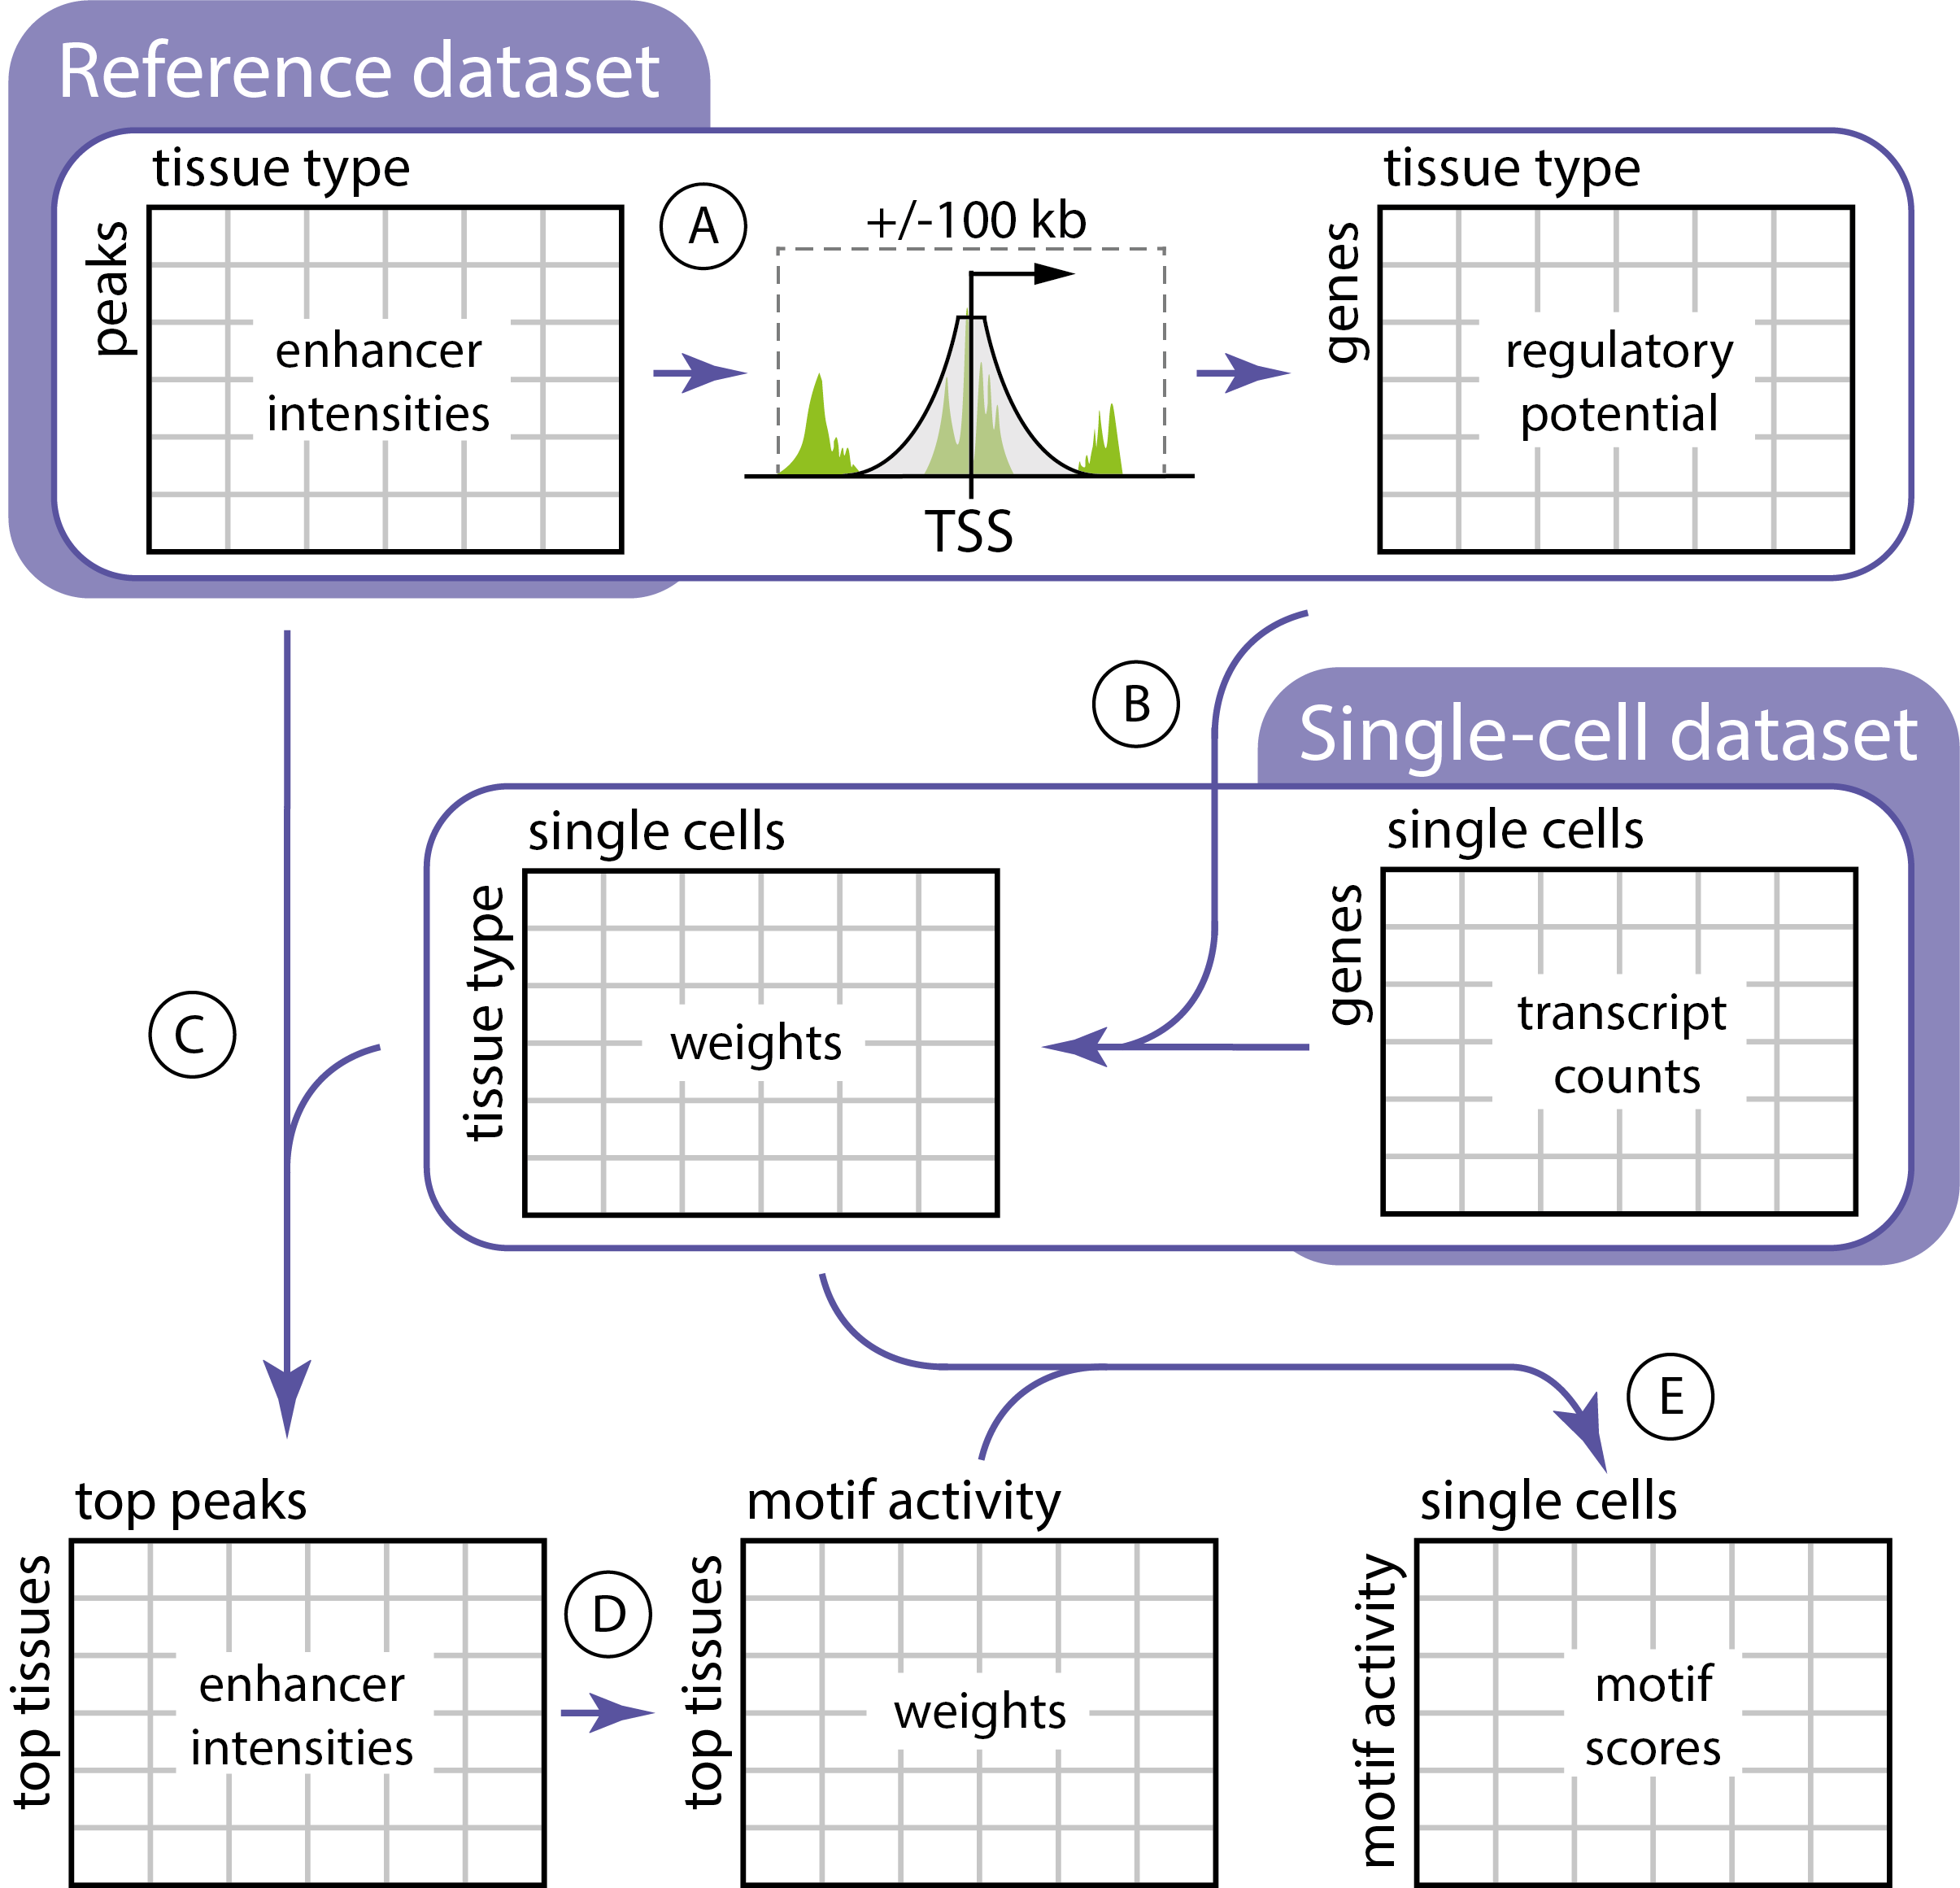
\includegraphics[width=1\linewidth]{ch.scepia/imgs/overview.png}
    \caption{TODO caption}
    \label{fig:enter-label}
\end{figure}

\noindent
Input:

\begin{itemize}
	\item reference Database:
    \begin{itemize}
        \item Let D be the reference database of H3K27ac or other genome-wide measurements related to enhancer "activity". D is represented as a matrix with dimensions (peaks x cell types).
    \end{itemize}
	\item Single-cell dataset:
    \begin{itemize}
        \item Let S be the single-cell dataset. S is represented as a matrix with dimensions (cells x genes).
    \end{itemize}
\end{itemize}

% TODO TISSUE TYPES OR CELL TYPES? Or sth else?

\noindent
This is how scepia works:

\begin{enumerate}[label=(\Alph*)]
    \item Convert the reference database matrix D into a database matrix of regulatory potential per gene (P).
    \begin{itemize}
        \item Let P be the regulatory potential. P is represented as a matrix with dimensions (genes x cell types)
        \item $P = f(D)$
        \item explain function f
    \end{itemize}
    \item Weigh each cell in the single-cell dataset (S) with regulatory potential (P) resulting in annotation matrix A.
    \begin{itemize}
        \item Let A be the cell type Annotation matrix. A is represented as a matrix with dimensions (cells x cell types)
        \item We do a lasso regression to infer the annotation weights: $S_i = P_i A_i + \lambda ||A_i||_1 +\epsilon$
        \item this is much more complex, as we first take cluster most common, then do it for each cell based on average neighbour gene expression, and finally, take the average cell type annotation of the neighbours..
    \end{itemize}
    \item Take the cell type annotations, and find the top most differential enhancers.
    \begin{itemize}
        \item $E_i = argmax_j(A_i)$
    \end{itemize}
    \item Do a motif scan
    \begin{itemize}
        \item matrix M
        \item We do a bayesian ridge regression to infer the motif weights: $S_i = P_i A_i + \lambda ||A_i||_2^2 +\epsilon$
    \end{itemize}
    \item dot product of annotation weights and motif scores F
    \begin{itemize}
        \item $F = S \cdot A$
    \end{itemize}
\end{enumerate}

% \begin{enumerate}
% 	\item H3K27ac Reference Database:
%     \begin{itemize}
%         \item Let R be the reference database of H3K27ac or other genome-wide measurements related to enhancer "activity."
%         \item R is represented as a matrix with dimensions (peaks x cell types).
%     \end{itemize}
%     \item scRNAseq Data:
%     \begin{itemize}
%         \item Let S be the scRNAseq data.
%         \item S is represented as a matrix with dimensions (cells x genes).
%     \end{itemize}
%     \item Regulatory Potential Matrix of H3K27ac Data:
%     \begin{itemize}
%         \item Let P be the regulatory potential matrix. 
%         \item It is a matrix with dimensions (genes x cell types) derived from the H3K27ac data.
%     \end{itemize}
%     \item Cell Type Annotation Matrix:
%     \begin{itemize}
%         \item Represented as A, it is a matrix with dimensions (cells x cell types), where values are weights or annotations indicating the association of cells with specific cell types.
%     \end{itemize}
%     \item Hypervariable Peaks Matrix from H3K27ac Signal:
%     \begin{itemize}
%         \item Represented as E, it is a matrix with dimensions (hypervariable peaks x cell types), which is a subset of matrix A and represents peaks with high variability in H3K27ac signal.
%     \end{itemize}
%     \item Cell Type Motif Activity Matrix:
%     \begin{itemize}
%         \item Represented as F, it is a matrix with dimensions (cell types x motifs) indicating the activity of motifs in different cell types
%     \end{itemize}
%     \item Single Cell Motif Activity Matrix:
%     \begin{itemize}
%         \item Represented as G, it is a matrix with dimensions (cells x motifs). The values in this matrix are obtained by taking the dot product of matrix D (cell type annotation) and matrix F (cell type motif activity). 
%     \end{itemize}
% \end{enumerate}

% $ ref = \begin{bmatrix}
% a_1 & a_2 & a_3 \\
% b_1 & b_2 & b_3 \\
% c_1 & c_2 & c_3 
% \end{bmatrix}  $

\section{Results}

\section{Discussion}

\subsection{Limitations}
\begin{itemize}
    \item Benchmark is bad. Benchmarking against a bad ground truth is stupid.
    \item 
\end{itemize}